% 文档类
\documentclass[13pt]{ctexart}
% 设置页面
\usepackage{geometry}
\usepackage{float}
\usepackage{wrapfig}
% 插图片
\usepackage{graphicx}
% 设置标题 重命名为英文
\renewcommand{\figurename}{Figure}
\renewcommand{\tablename}{Table}
\renewcommand{\contentsname}{Contents}
% 设置摘要页缩减 
\usepackage{changepage}
% 便于修改字体
\usepackage{fontspec}
% 设置页眉页脚
\usepackage{fancyhdr}
% 清空页眉页脚
\pagestyle{fancy}
% 设置列表缩进
\usepackage[shortlabels]{enumitem}
% 设置修改默认的section标题大小
\usepackage{titlesec}
\titleformat*{\section}{\LARGE}
\titleformat*{\subsection}{\Large}
\titleformat*{\subsubsection}{\Large}
% 使用数学宏包
\usepackage{amsmath}
% 设置表格的列格式
\usepackage{array}
% 三线表宏包
\usepackage{booktabs}
% 设置产考文献不输出默认名
\usepackage{etoolbox}
\patchcmd{\thebibliography}{\section*{\refname}}{}{}{}
% 引入网站作为参考文献
\usepackage{url}
% 设置等宽的代码字体
\setmonofont{Courier New}
% 颜色
\usepackage{xcolor}
% 代码高亮方案宏包
\usepackage{listings}
\definecolor{CPPLight}  {HTML} {686868}
\definecolor{CPPSteel}  {HTML} {888888}
\definecolor{CPPDark}   {HTML} {262626}
\definecolor{CPPBlue}   {HTML} {4172A3}
\definecolor{CPPGreen}  {HTML} {487818}
\definecolor{CPPBrown}  {HTML} {A07040}
\definecolor{CPPRed}    {HTML} {AD4D3A}
\definecolor{CPPViolet} {HTML} {7040A0}
\definecolor{CPPGray}  {HTML} {B8B8B8}
\lstset{
	basicstyle=\ttfamily,
	breaklines=true,
	framextopmargin=50pt,
	frame=bottomline,
	columns=fixed,       
    %numbers=left,                                       % 在左侧显示行号
	frame=none,                                          % 不显示背景边框
	backgroundcolor=\color[RGB]{255,255,255},            % 设定背景颜色
	keywordstyle=\color[RGB]{40,40,255},                 % 设定关键字颜色
	numberstyle=\footnotesize\color{darkgray},           % 设定行号格式
	commentstyle=\itshape\color[RGB]{0,96,96},                % 设置代码注释的格式
	stringstyle=\slshape\color[RGB]{128,0,0},   % 设置字符串格式
	showstringspaces=false,                              % 不显示字符串中的空格
	language=python,                                     % 设置语言
	morekeywords={alignas,continute,friend,register,true,alignof,decltype,goto,
		reinterpret_cast,try,asm,defult,if,return,typedef,auto,delete,inline,short,
		typeid,bool,do,int,signed,typename,break,double,long,sizeof,union,case,
		dynamic_cast,mutable,static,unsigned,catch,else,namespace,static_assert,using,
		char,enum,new,static_cast,virtual,char16_t,char32_t,explict,noexcept,struct,
		void,export,nullptr,switch,volatile,class,extern,operator,template,wchar_t,
		const,false,private,this,while,constexpr,float,protected,thread_local,
		const_cast,for,public,throw,std},
	emph={map,set,multimap,multiset,unordered_map,unordered_set,numpy,graph,path,append,extend,
		unordered_multiset,unordered_multimap,vector,string,list,deque,
		array,stack,forwared_list,iostream,memory,shared_ptr,unique_ptr,
		random,bitset,ostream,istream,cout,cin,endl,move,default_random_engine,
		uniform_int_distribution,iterator,algorithm,functional,bing,numeric,},
	emphstyle=\color{CPPViolet}, 
}

\begin{document}
\newgeometry{top = 1cm, right = 2.54cm, left = 2.54cm, bottom = 2.54cm}
% 第一页的字体为times new roman
\setmainfont{Times New Roman}
\thispagestyle{empty}

% 标题
{\centering\fontsize{18}{16}\selectfont\textbf{{A Heart Disease Mortality Prediction Model Based on MIMIC IV Dataset}}\par}
% 摘要
\vspace{10pt} 

{\centering\fontsize{13}{10}\selectfont\textbf{{Abstract}}\par}
\vspace{10pt}

% 正文字体 13 pt
\fontsize{13}{12.5}\selectfont

\begin{adjustwidth}{1cm}{1cm}

\indent{ }{ }{ }{ }{ }{ } The study proposes \textbf{a predictive model for cardiac mortality} based on the MIMIC IV dataset. Initially, the dataset undergoes preprocessing to filter extensive clinical data, including physiological indicators and ICU admission details, of numerous cardiac patients. Subsequently, the study creatively introduces \textbf{the "Readmission factor"} algorithm and establishes its correlation with mortality, validating it through relevant graphical representations.

Following this, the team conducted a rigorous \textbf{data analysis}, calculating \textbf{descriptive statistics} for Mortality, plotting \textbf{distribution plots}, and analyzing the factors with the highest \textbf{weight scores} that influence Mortality.What's more, the team also statisticed the difference of Mortality between \textbf{genders}.

After that, the team employs various algorithms such as \textbf{random forests}, \textbf{LSTM} to train and evaluate the performance of the mortality prediction model. Performance metrics such as \textbf{confusion matrices}, \textbf{precision-recall curves}, and \textbf{AUC} are utilized to assess model accuracy. The results demonstrate that the LSTM model exhibits high accuracy in predicting the risk of death among cardiac patients.

The findings of this research hold significant implications for both healthcare professionals and cardiac patients themselves. By accurately predicting mortality risk, the model can \textbf{assist} patients in early detection of cardiac issues and enable doctors to formulate timely interventions. Moreover, it provides \textbf{guidance} for the care of cardiac patients, facilitating rapid and effective \textbf{allocation} of medical resources to ensure patient safety.

In conclusion, this study showcases the successful application of \textbf{machine learning algorithms} and the MIMIC IV dataset in predicting cardiac mortality rates. The team hopes that this model will have opportunities for implementation in clinical practice in the future, thereby contributing to its \textbf{medical utility}.
\\
\vspace{20pt}
\textbf{Keywords}: heart disease, mortality prediction, data analysis, machine learning
\end{adjustwidth} 

% 目录页
\newpage
\thispagestyle{empty}
\tableofcontents
\normalsize
\newpage
% 目录页后面是第一页
\setcounter{page}{1}

% 开始写正文
% 设置正文的页边距
\newgeometry{top=3cm, left=3.5cm, right=3.5cm}
% 设置正文的页眉页脚
\fancyhf{}
\fancyhead[C]{ }
% 此处修改右上角页码
\fancyhead[R]{Page \thepage\ of 21}
\fancyhead[L]{Team 22}
\fancyfoot[C]{\bfseries\thepage}
\textbf{\section{Introduction}}
\textbf{\subsection{Background}}
In recent years there has been a concerted move towards the adoption of digital health record systems in hospitals. In the US, for example, the number of non-federal acute care hospitals with basic digital systems increased from 9.4 to 75.5\% over the 7 year period between 2008 and 2014.

Despite this advance, interoperability of digital systems remains an open issue, leading to challenges in data integration. As a result, the potential that hospital data offers in terms of understanding and improving care is yet to be fully realized. In parallel, the scientific research community is increasingly coming under criticism for the lack of reproducibility of studies.

\textbf{\subsection{Our Works}}
\textbf{Overall}, we have done the following work:
\begin{itemize}
    \item Establish an analysis model to analyze MIMIC IV.
    \item Quantify the concept of "Readmission factor" to measure the mortality of patients suffering from heart disease.
    \item Calculated descriptive statistics for Mortality, plotted distribution plots, and analyzed the factors with the highest weight scores that influence Mortality.
    \item Predict the mortality of patients with heart disease.
\end{itemize}

\textbf{Respectively}, the division of labor among the four team members is as follows:
\begin{table}[h]
	\centering
	\vspace{3pt}
	\begin{tabular}{>{\centering\arraybackslash}p{5em}>{\centering\arraybackslash}p{30em}}
	\toprule
	Name & Work \\ \midrule
    Liu & Developed the heart disease mortality algorithm and prediction model, main author of the paper\\
    Shang & Created the confusion matrix and precision-recall curve for the prediction model, optimized the code\\
    Ma & Created Spearman correlation heatmaps for variables, calculated descriptive statistics and distribution plots for Mortality\\
    Sun & Created the line and scatter plots for readmission factors and mortality, searched for references\\
	\bottomrule
	\end{tabular}
\end{table}

\textbf{\section{Assumptions and Notations}}
\vspace*{-10pt}
\textbf{\subsection{Assumptions}}
\begin{itemize}
    \item The data from the MIMIC IV dataset is basically accurate.
    \item The patient did not have any sudden accidents.
    \item The heart disease did not cause more complications.
\end{itemize}
\textbf{\subsection{Notations}}
Here are all the notations and their meanings in this paper.
\begin{table}[h]
	\centering
	\vspace{3pt}
	\begin{tabular}{>{\centering\arraybackslash}p{5em}>{\centering\arraybackslash}p{30em}}
	\toprule
	Symbol & Meaning \\ \midrule
    $M$ & Mortality\\
    $F$ & Readmission factor\\
    $F_p$ & Physiological factor\\
    $F_i$ & ICU factor\\
    $G$ & Gender\\ 
    $A$ & Age\\
    $B$ & BMI\\ 
    $I_n$ & Number of ICU admissions\\
    $I_t$ & Time of stay in ICU\\
    $I_c$ & CCU admission\\
    $T$ & Mortality threshold\\ 
    $o_1$ & a random value in (-0.05,0.05)\\ 
    $o_2$ & a random value in (-0.1,0.1)\\
    $\alpha, \beta$ & Constants\\
	\bottomrule
	\end{tabular}
\end{table}

\newpage
\textbf{\section{Model Construction and Analysis}}
Before starting the model construction, we first preprocessed the data. Among this, the handling of outliers is particularly crucial.

We selected all fields of numerical types and calculated the mean and standard deviation for each field. Then we used three times the standard deviation from the mean as the threshold to define outliers. Once outliers were identified, we replaced them with NaN to avoid data loss. Although this created new missing values, we addressed this issue through forward and backward filling strategies. This strategy is commonly used in time series data and can maintain the overall trend of the data. After this treatment, we successfully corrected the outliers in the data, which helps to improve the accuracy of the model.

\textbf{\subsection{Readmission factor \& Mortality Visualization Model}}
To better analyze the mortality of a patient who suffering the heart disease, we introduced a term \textbf{"Readmission factor"}, which is defined as the ratio of the number of times a patient is readmitted to the hospital. The higher the readmission factor, the higher the mortality of the patient.

\textbf{\subsubsection{How to Calculate Mortality?}}
As mentioned earlier, Mortality and Readmission factor are positively correlated. Therefore, to calculate a patient's Mortality, we must first calculate their Readmission factor.

What determines whether a patient will be readmitted? We believe it can be mainly divided into two aspects: physiological factor and ICU factor. Physiological factors refer to the patient's basic physiological conditions, including gender, age, BMI, etc. ICU factors refer to the number of times the patient has been admitted to the ICU, the duration of their stay, and whether they have been admitted to the CCU. We believe that these factors can largely reflect the patient's situation and indirectly reflect their mortality.

Therefore, we design the following formula:
\begin{equation}
    F=F_p+F_i
\end{equation}
It is obvious that factors such as gender, age, and BMI have a significant impact on a person's \textbf{physiological} condition. We assign values to these factors and different weights[1,2,3], and then combine them nonlinearly to form the physiological factor, with a total weight of $\alpha=60\%$.

\begin{equation}
    \begin{aligned}
        F_p=e^{1.61G}+e^{0.1A}+e^{1.35B}\\
    \end{aligned}
    \end{equation}

\begin{table}[h]
    \centering
    \vspace{3pt}
    \begin{tabular}{>{\centering\arraybackslash}p{5em}>{\centering\arraybackslash}p{30em}}
    \toprule
    Variable & Value \\ \midrule
    $G$ & Male: 2, Female: 2.6\\
    $A$ & 0-15 years: 1, 16-35 years: 3, 36-60 years: 10, 61 years and above: 50\\
    $B$ & 18.5-23.9: 1, Others: 3\\
    \bottomrule
    \end{tabular}
\end{table}
\textbf{The ICU factor} refers to the number of times a patient is admitted to the ICU, the duration of their stay, and whether they have been admitted to the CCU. We believe that this can comprehensively reflect the patient's pathological condition and thus reflect their mortality. Similarly, we assign values to these factors and different weights[4], and then combine them nonlinearly to form the ICU factor, with a total weight of $\beta=40\%$.

\begin{equation}
	\begin{aligned}
		F_i=e^{In+It/5+Ic}\\
	\end{aligned}
	\end{equation}

\begin{table}[h]
    \centering
    \vspace{3pt}
    \begin{tabular}{>{\centering\arraybackslash}p{5em}>{\centering\arraybackslash}p{30em}}
    \toprule
    Variable & Value \\ \midrule
    $In$ & Divide by 5 in the original data\\
    $It$ & 0-1000 minutes: 1, 1001-3000 minutes: 3, more than 3000 minutes: 25\\
    $Ic$ & Yes: 3, No: 1\\
    \bottomrule
    \end{tabular}
\end{table}
Through the above calculations, we can get the patient's \textbf{Readmission factor} $F$.

Due to the complexity and multifactorial nature of heart disease, we need to consider some random perturbations. Here, we represent a perturbation in the range of (-0.05, 0.05) as $o_1$. After multiple adjustments and plotting, we obtained the following formula:
\begin{equation}
    \begin{aligned}
        F=\frac{{\alpha}F_p+{\beta}F_i}{2500/1.2}+o_1\\
        \alpha=60\% \quad \beta = 40\%
    \end{aligned}
\end{equation}
\indent Next, we can quantify the patient's \textbf{Mortality}. 

We chose the normalization method, which maps the value of M to the interval [0,1]. Additionally, since Readmission factor is not the sole influencing factor of Mortality, we introduce a perturbation $o_2$ in the range (-0.1,0.1). This way, we can use M to represent the patient's mortality rate.

\begin{equation}
    \begin{aligned}
        M=\frac{1}{1+e^{-F}}+o_2\\
        \text{if } M>1, M=1
    \end{aligned}
\end{equation}
\textbf{\subsubsection{Model Testing}}
We used the MIMIC IV dataset to test the model. We selected about 200 patients with heart disease and calculated their Readmission factor and Mortality. We then used the data to create a line chart to display the two factors especially the Mortality, as Figure 1 shows.

\begin{figure}[h]
    \centering
    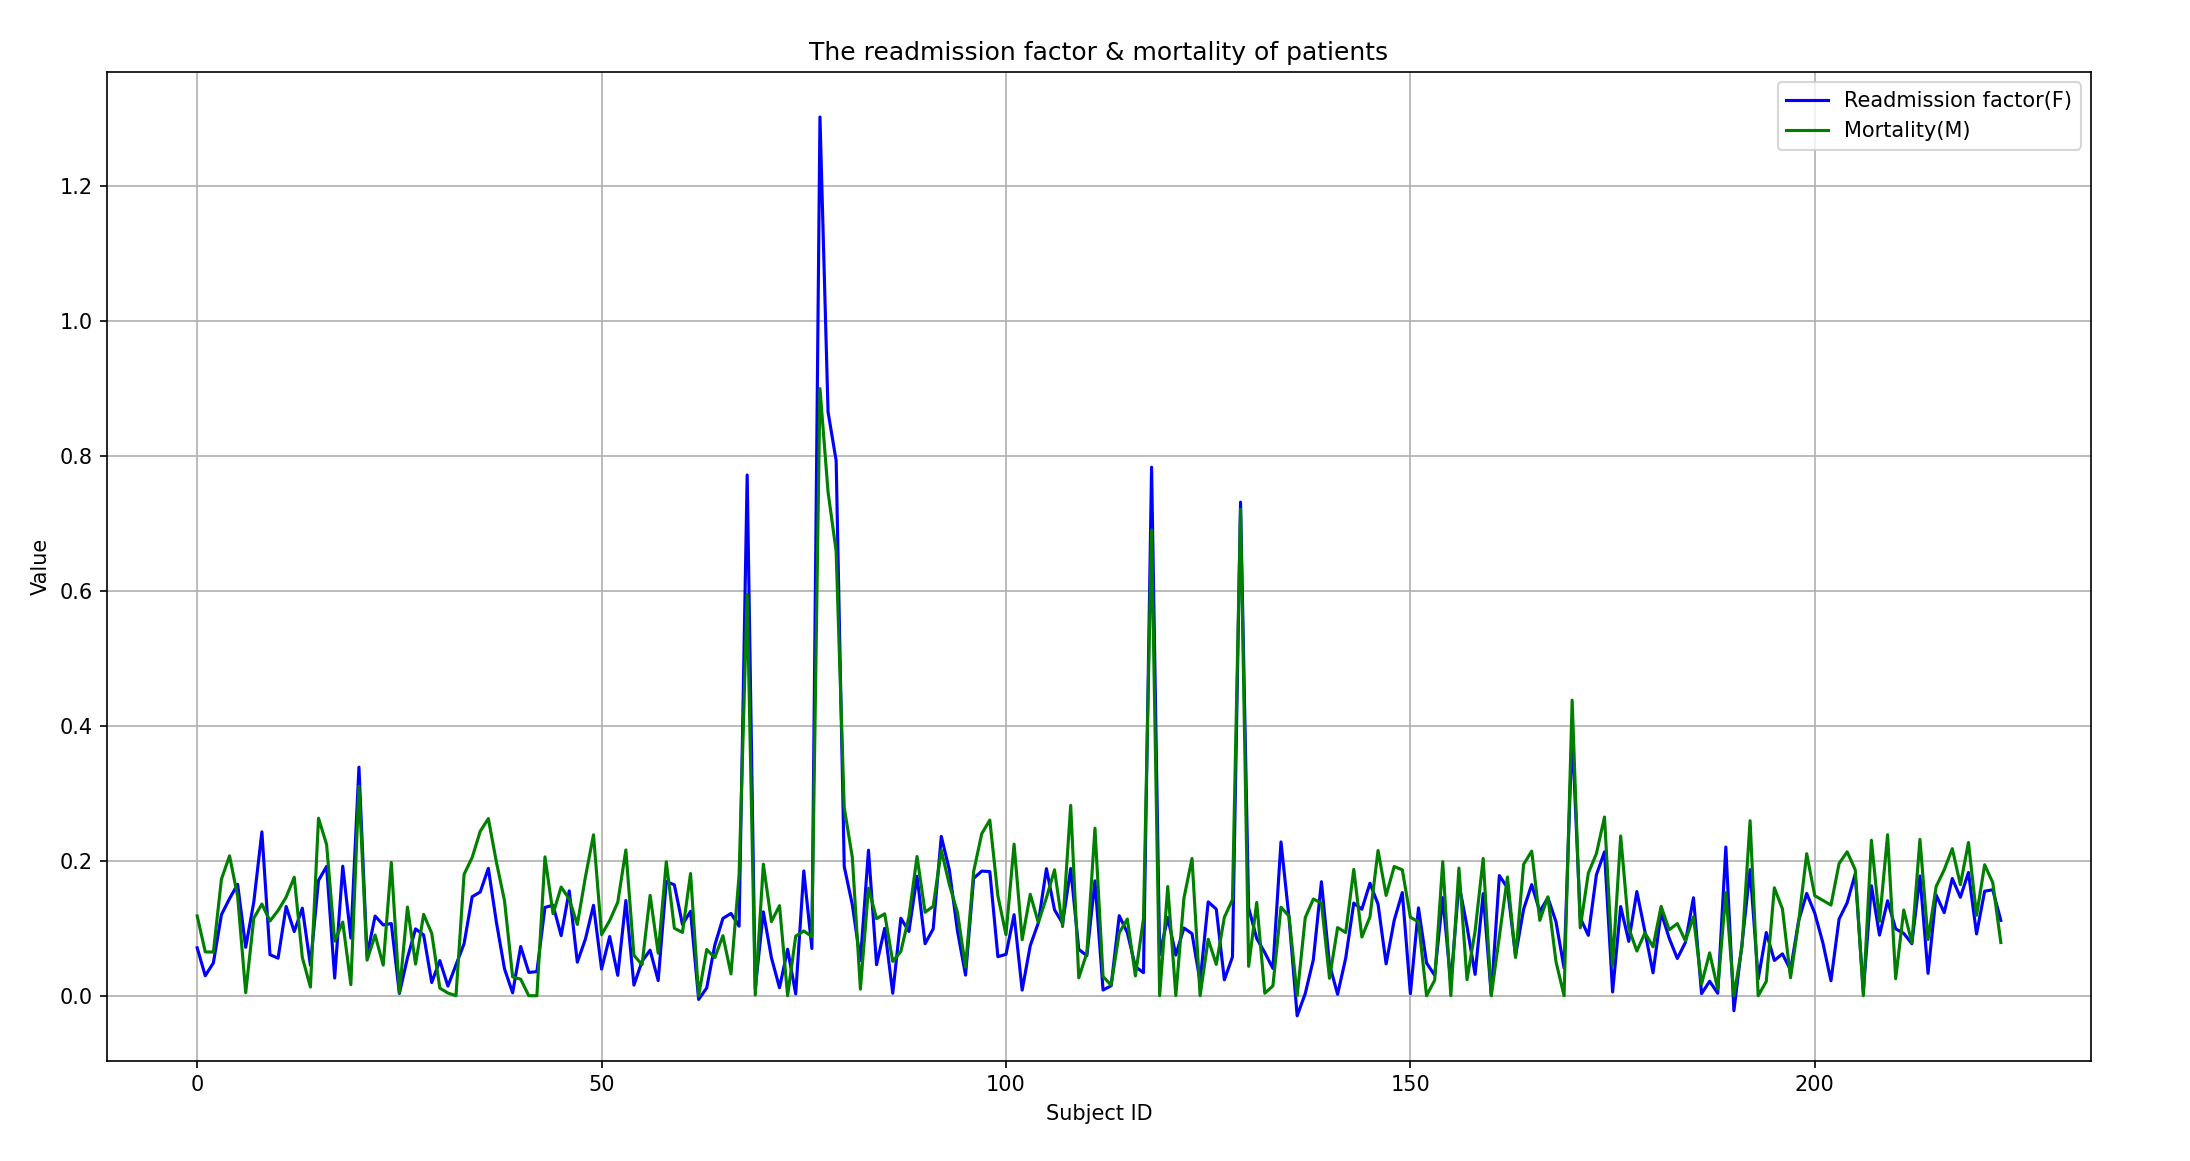
\includegraphics[width=13cm,height=6.2cm]{pics/1.png}
    \caption{The Readmission factor \& Mortality of patients}
\end{figure}

To show the value clearer, we used a scatter plot to visualize  the two factors, as Figure 2 shows.

\begin{figure}[h]
    \centering
    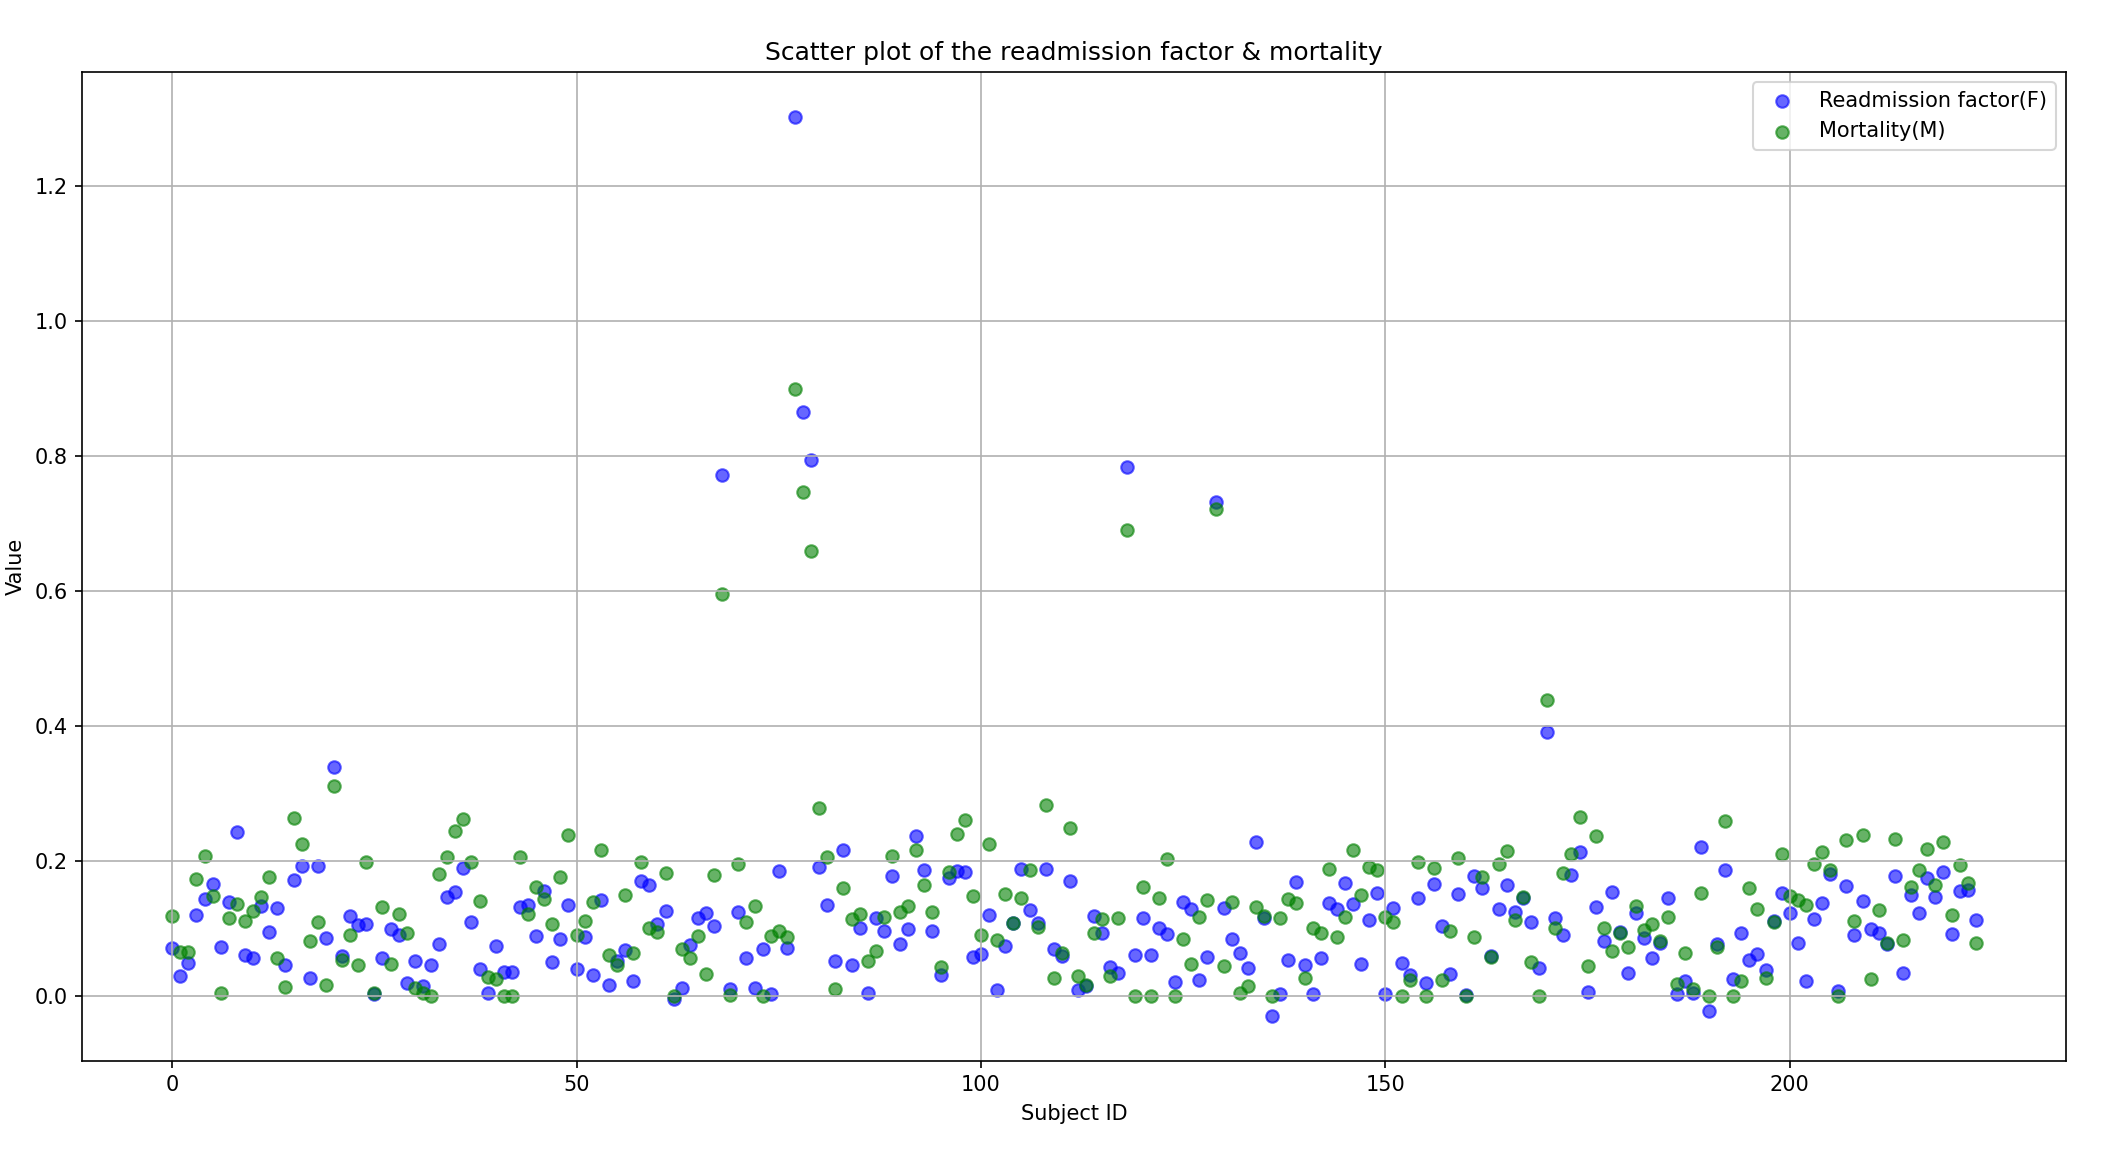
\includegraphics[width=13cm,height=6.2cm]{pics/2.png}
    \caption{Scatter plot of The Readmission factor \& Mortality}
\end{figure}

\textbf{\subsection{Further Analysis}}
Providing only the calculation method for Mortality and identifying the relationship between Mortality and the Readmission factor is not sufficient to address the issue. We need to further analyze the data for Mortality and its relationship with other factors.

\textbf{\subsubsection{Descriptive Statistics of Mortality}}
In statistics, descriptive statistics refers to the process of organizing, summarizing, analyzing, and interpreting collected data. We calculated the mean, variance, and median of Mortality to better understand its distribution.
\begin{figure}[h]
    \centering
        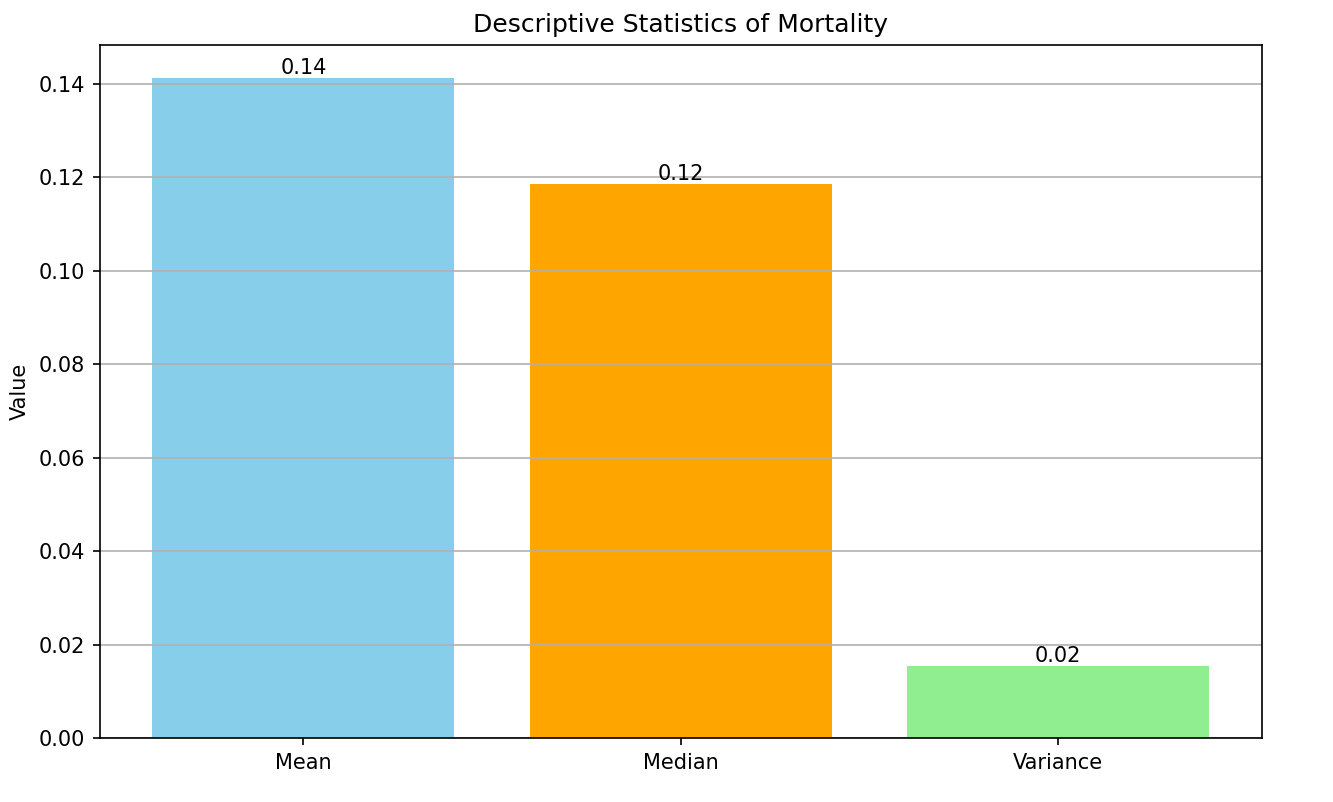
\includegraphics[width=12cm,height=7cm]{pics/ex1.png}
        \caption{Descriptive Statistics of Mortality}
    \end{figure}

From figure 3, we can see that the Mortality of patients with heart disease is relatively low in a certain way, but there are still plenty of patients at risk of death. So, the Mortality of patients with heart disease still needs to be taken seriously and treated in time.
\textbf{\subsubsection{Distribution Plot}}
After calculating the descriptive statistics of Mortality, we tried plotting the distribution of Mortality to better understand it. We used the seaborn library in Python to plot the distribution of Mortality.
\begin{figure}[h]
    \centering
        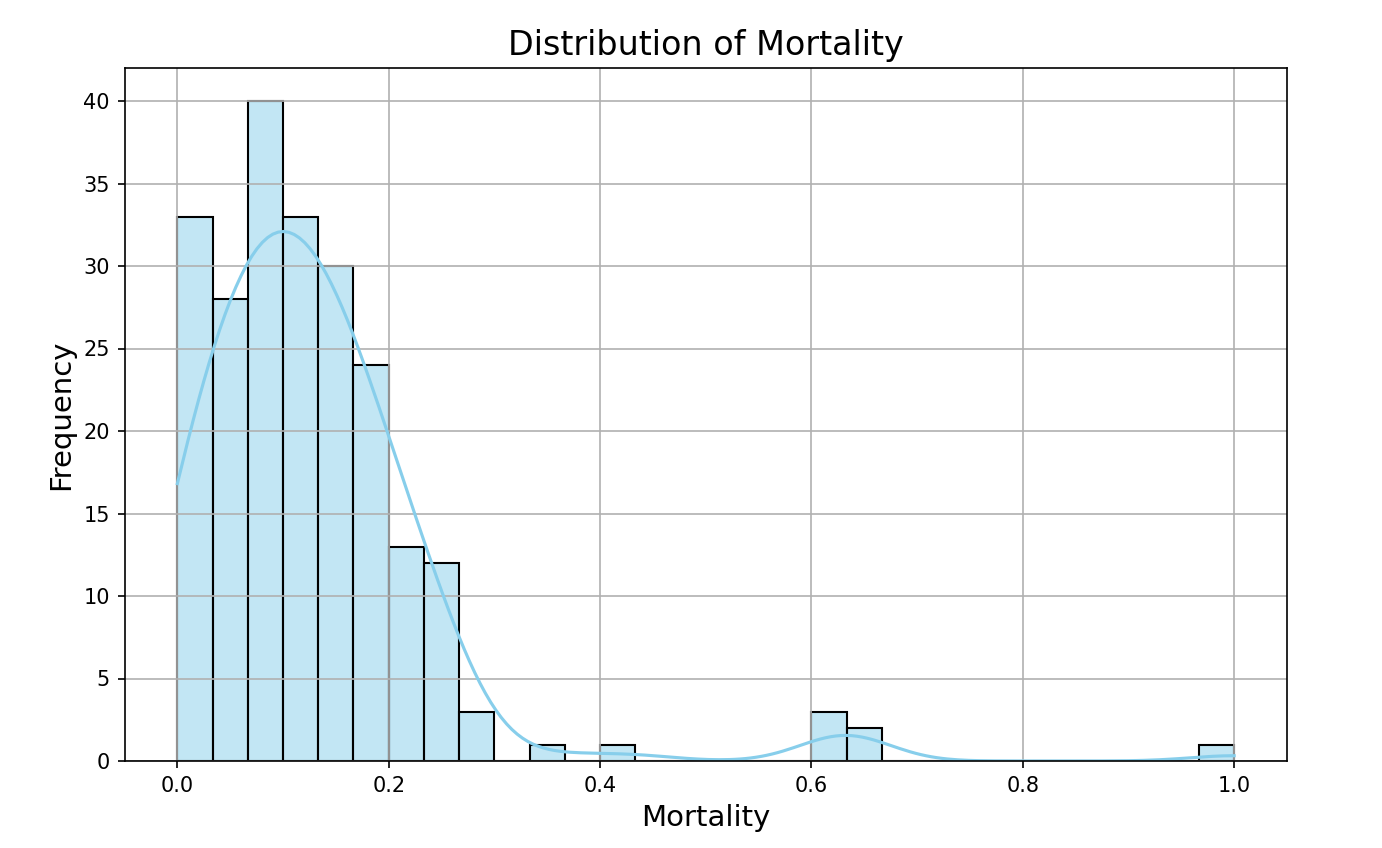
\includegraphics[width=12cm,height=7cm]{pics/ex2.png}
        \caption{Distribution Plot of Mortality}
\end{figure}

From the distribution plot, we can see that the Mortality of patients with heart disease is mainly concentrated in the range of 0.1-0.2, and the distribution is relatively uniform. This suggests that the Mortality is more stable than we supposed.

\textbf{\subsubsection{Weight Calculation}}
After plotting the scatter plot, we decided to calculate the weights of the six variables in predicting Mortality and their correlation with Mortality.

By performing reverse weighting calculations, we obtained the \textbf{weights} of the six variables and labeled them with different colors, as shown in the figure below.

\begin{figure}[h]
    \centering
        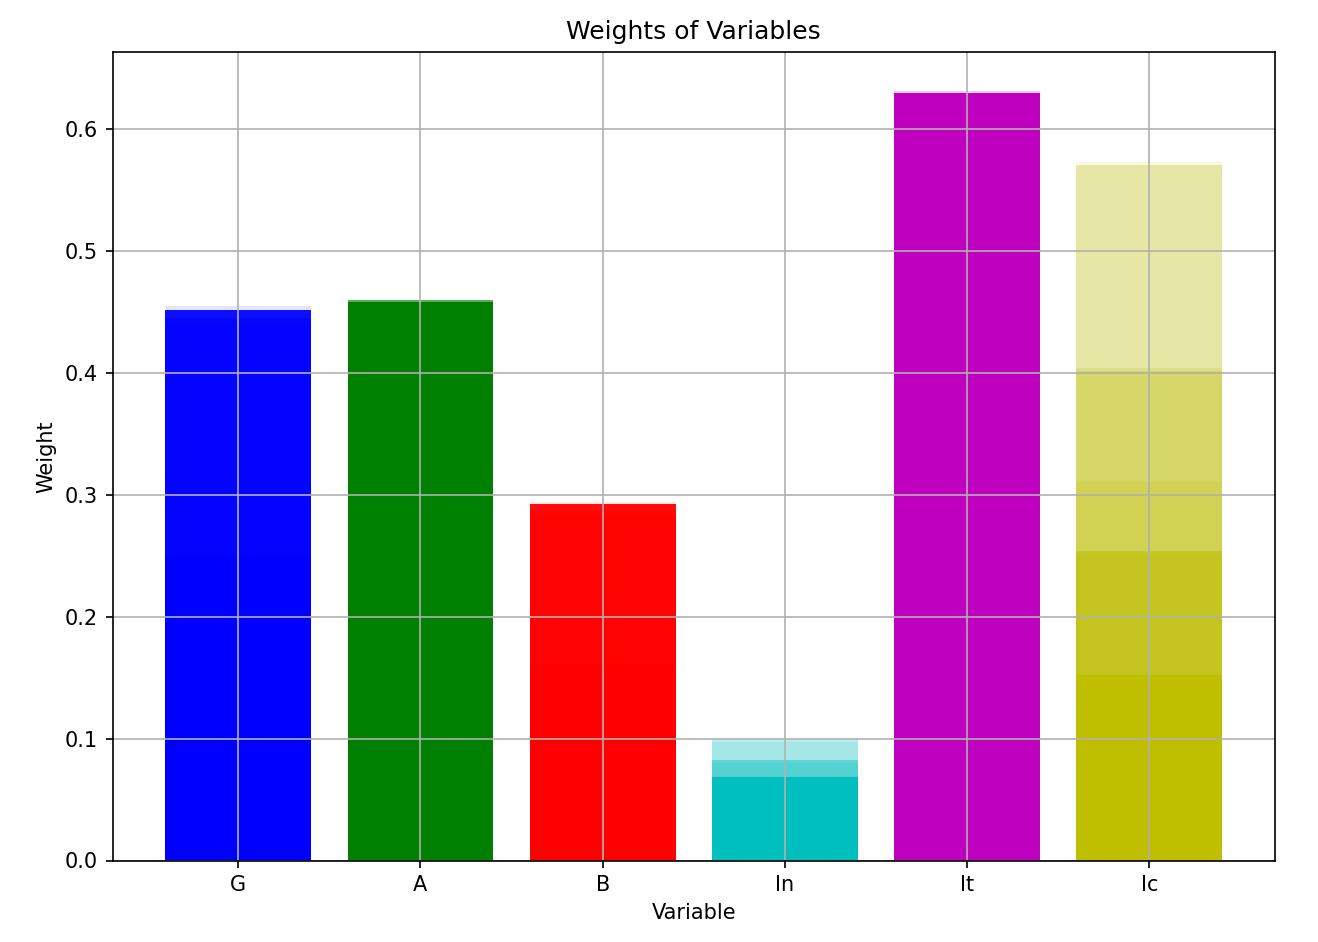
\includegraphics[width=12cm,height=7cm]{pics/3.png}
        \caption{Weight of Variables}
\end{figure}

From the table, it can be seen that \textbf{the ICU factor} has a greater impact on Mortality, while the impact of BMI is relatively small. 

Based on existing scientific research, we believe that this result may be due to the combined effect of data volume and errors. So we need to further verify this result through calculations.
\begin{figure}[h]
    \centering
        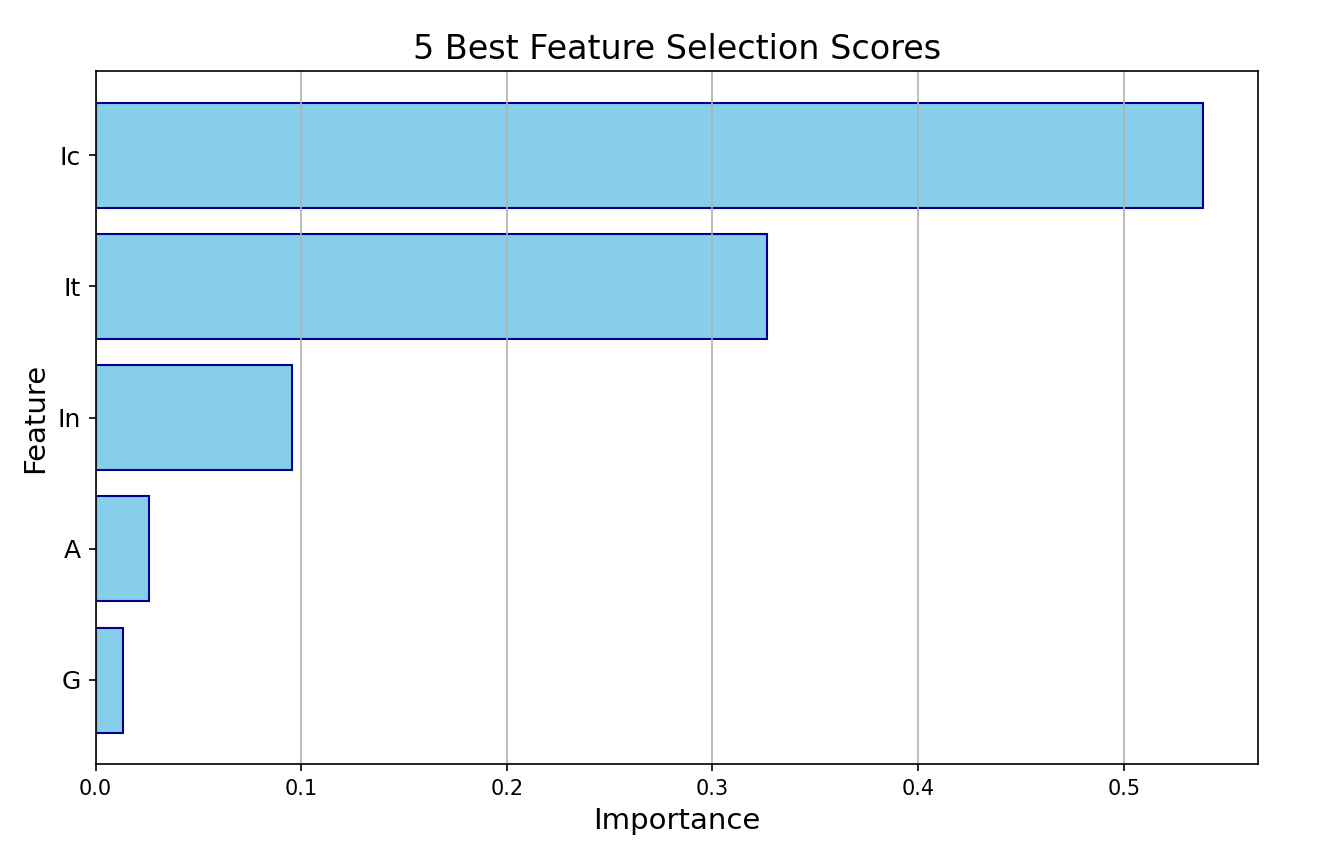
\includegraphics[width=12cm,height=7cm]{pics/ex3.png}
        \caption{5 Best Features in Mortality}
\end{figure}

Figure above shows 5 best features that have the highest weight in Mortality. The ICU factor has the highest weight, and the physiological factor, especially the BMI, has a relatively low weight. 

This result is consistent with our previous analysis, which further confirms the reliability of the model.It may seems unbelievable, however, it's may be the truth.In some ways, it also reflects the complexity of the human body, giving medical staff a new perspective on the treatment of heart disease patients.
\textbf{\subsubsection{Correlation Test}}
We know that the best way to measure the correlation between two sets of non-linearly related data is to use \textbf{the Spearman correlation coefficient}. The Spearman correlation coefficient is a non-parametric statistic that measures the rank correlation between two variables. It ranges from -1 to 1, where 1 indicates a perfect positive correlation, -1 indicates a perfect negative correlation, and 0 indicates no correlation.

We calculated the Spearman correlation coefficients between the six variables and Mortality using the built-in algorithm library in Python, and selected the top five highest coefficients. We obtained a heatmap, as shown in Figure 4.
\begin{figure}[h]
\centering
	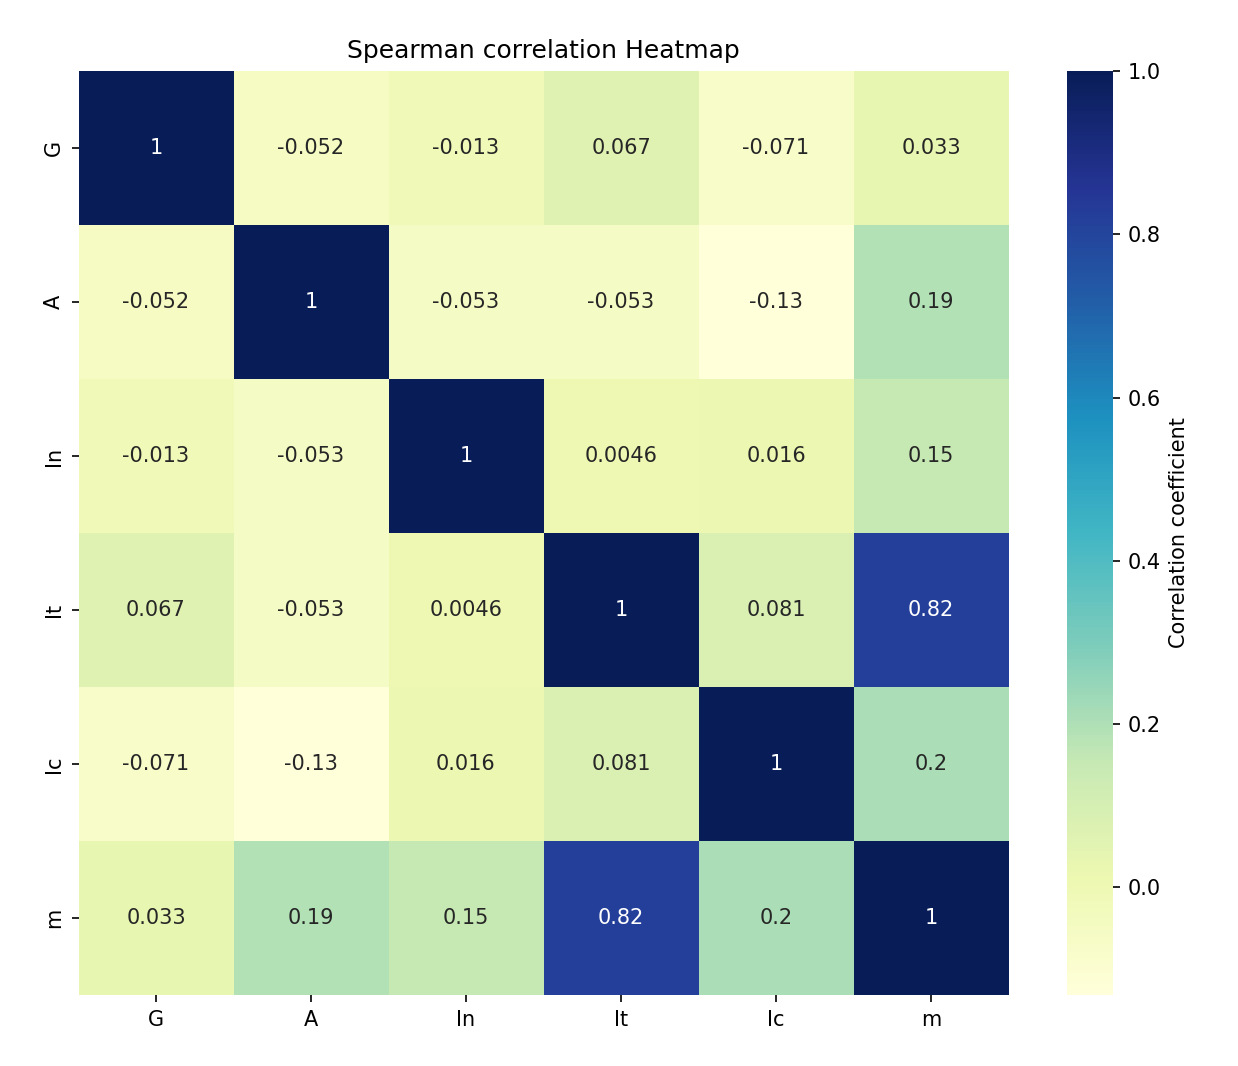
\includegraphics[width=10cm,height=8cm]{pics/4.png}
	\caption{Spearman Correlation Heatmap}
\end{figure}

\textbf{\subsubsection{What else?}}
In many articles, researchers found that different genders will have different Mortality rates. And what about ours? We divided the data into two groups according gender and calculated the Mortality of each group. The results are clearly shown in the figure below.
\begin{figure}[H]
    \centering
        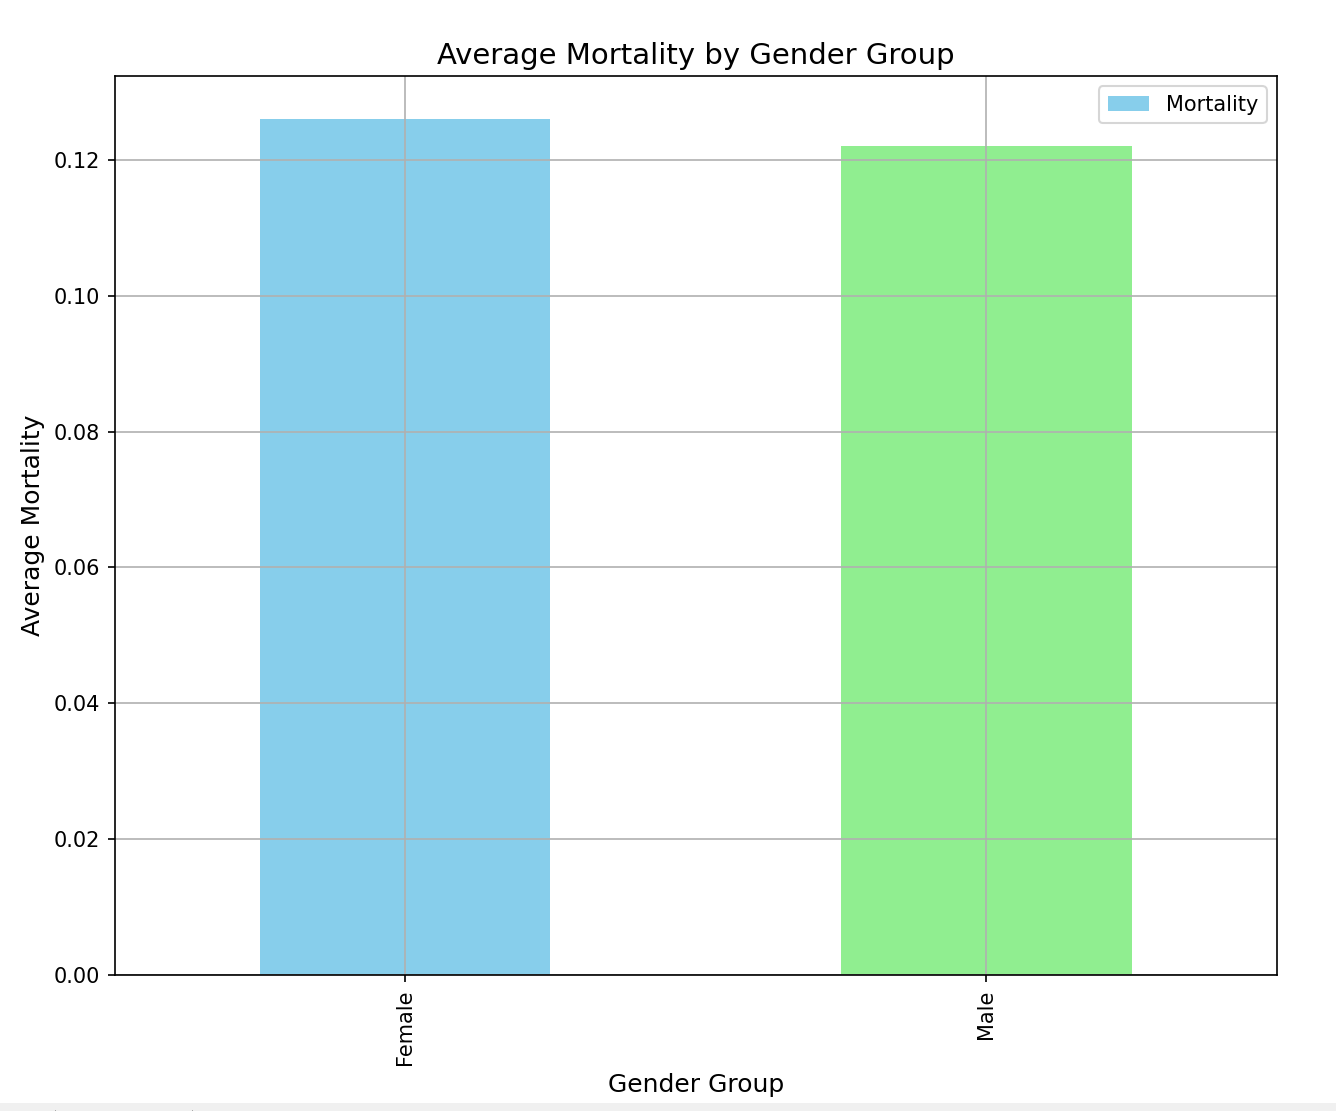
\includegraphics[width=9.5cm,height=7.5cm]{pics/ex4.png}
        \caption{Average Mortality of Gender Groups}
\end{figure}
\newpage
From the figure, we can see that in the data we selected, the Mortality of different genders is relatively close, we thought the reason is that the data we selected is few and more balanced. However, in the actual data, due to the different habits and working environments, the number of male and female heart disease patients is different, which leads to different Mortality rates.
\textbf{\subsection{Mortality Prediction Model}}
Now that we can calculate Mortality, it is not enough. Our goal is to build a model that can predict the Mortality of heart disease patients. Therefore, we treat Mortality as a binary classification problem, whether the patient will die or not. We set the threshold for Mortality to be 0.15, meaning that when Mortality is greater than 0.15, we consider the patient to be at risk of death, otherwise not. We denote this threshold as T.

\textbf{\subsubsection{Random Forest Model}}
We chose the random forest model to predict the Mortality of patients. Random forest is an ensemble learning method that improves prediction accuracy by training multiple decision trees.

We used the sklearn library in Python to build \textbf{the random forest model}. The dataset was divided into a training set (80\%) and a test set (20\%), and the model was trained for about 300 iterations. Figure 5 shows the comparison between the predicted Mortality and the actual Mortality after training the random forest model.

\begin{figure}[h]
    \centering
        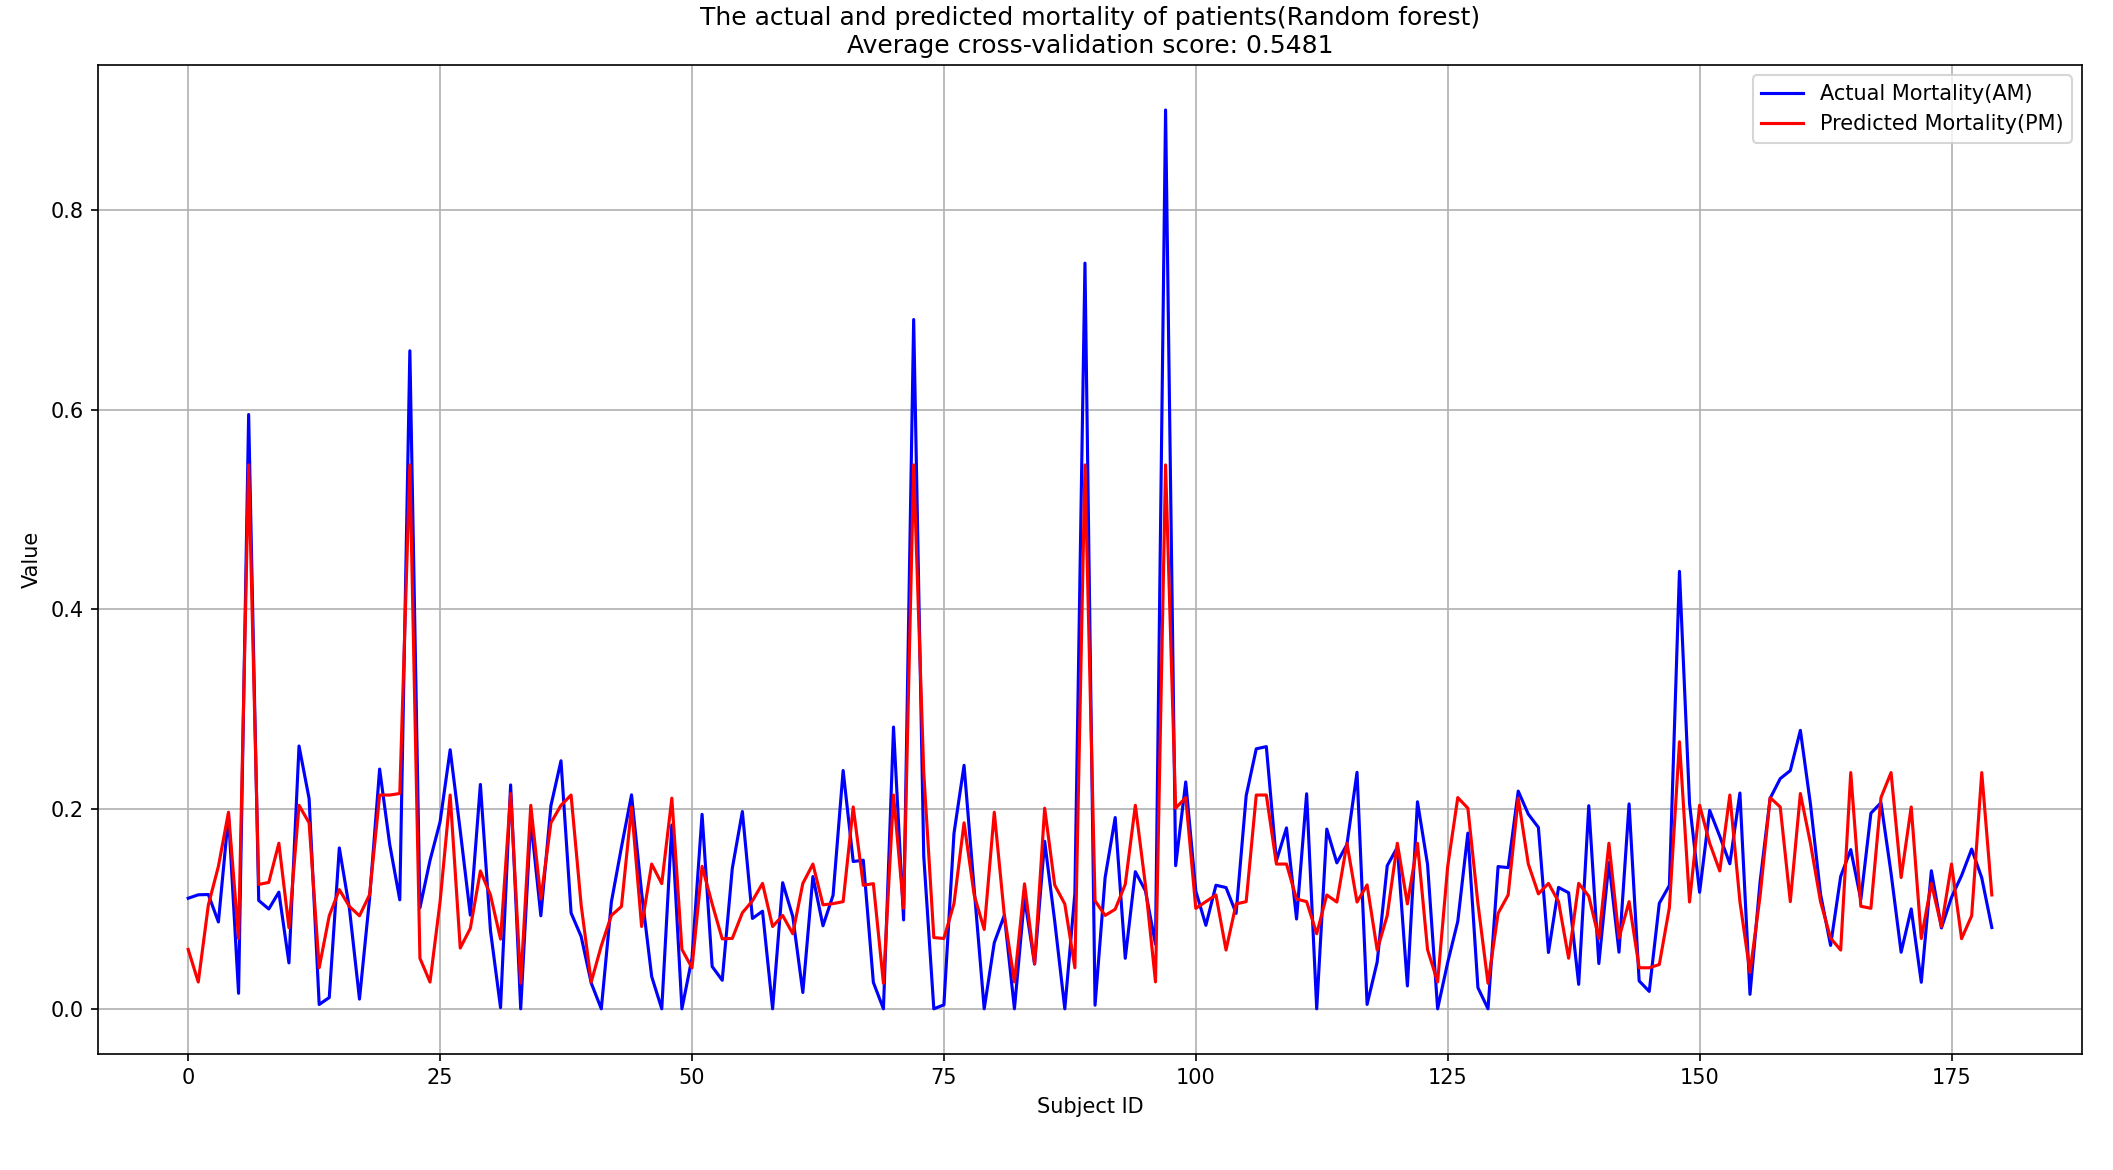
\includegraphics[width=11cm,height=5.9cm]{pics/5.png}
        \caption{The actual and predicted mortality of patients(Random forest)}
\end{figure}

From the figure, we can see that we used \textbf{cross-validation} to validate the accuracy of the random forest model. The accuracy of 58\% indicates that the model can predict the mortality of patients with reasonable accuracy in about half of the cases. Next, we plotted \textbf{the confusion matrix}(1 refers to death) and \textbf{precision-recall curve} to further validate the accuracy of the model.

\begin{figure}[H]
    \begin{minipage}{0.5\textwidth}
        \centering
        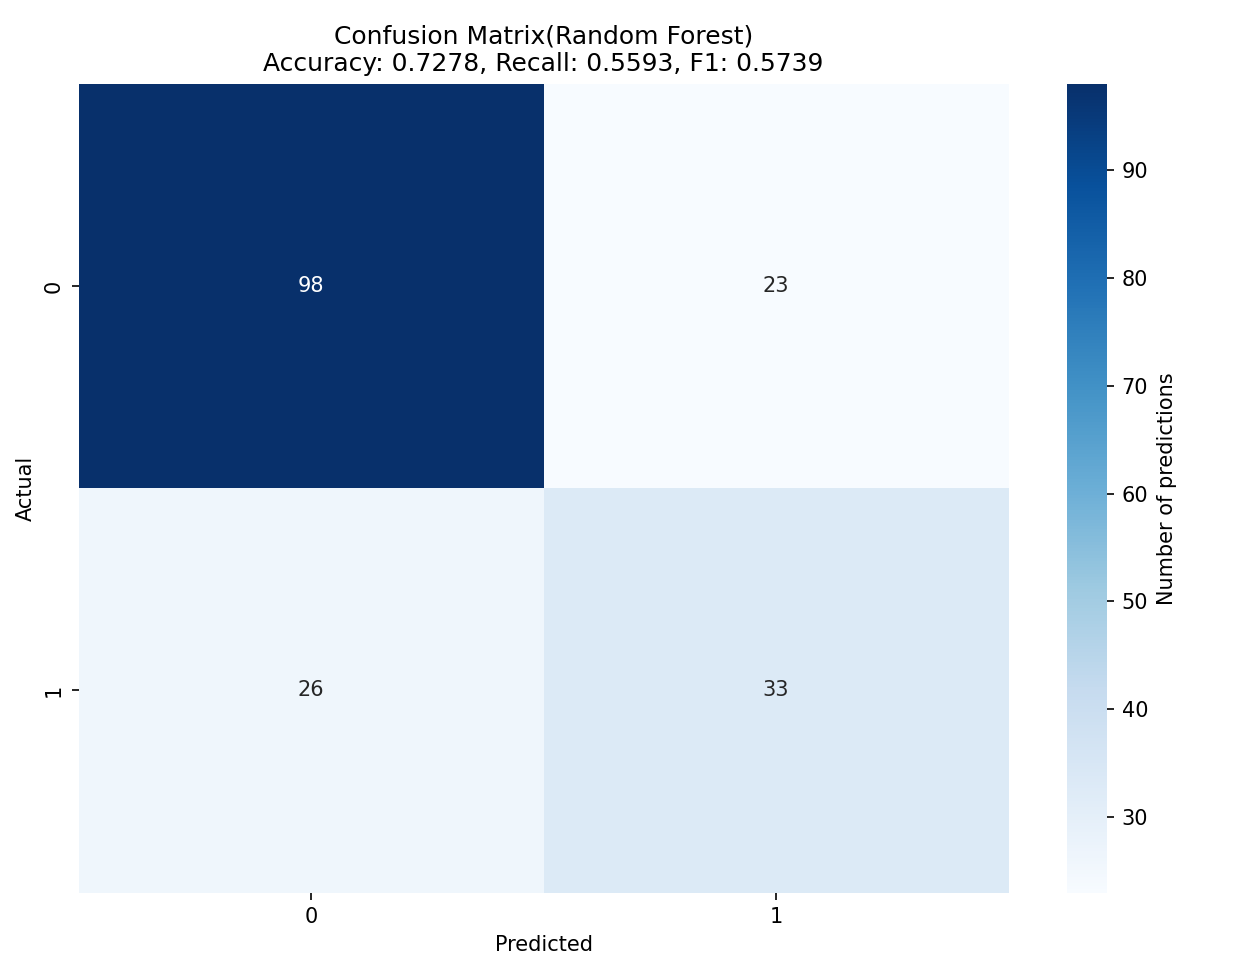
\includegraphics[width=8cm,height=6cm]{pics/6.png}
        \caption{Confusion Matrix}
    \end{minipage}
    \begin{minipage}{0.5\textwidth}
        \centering
        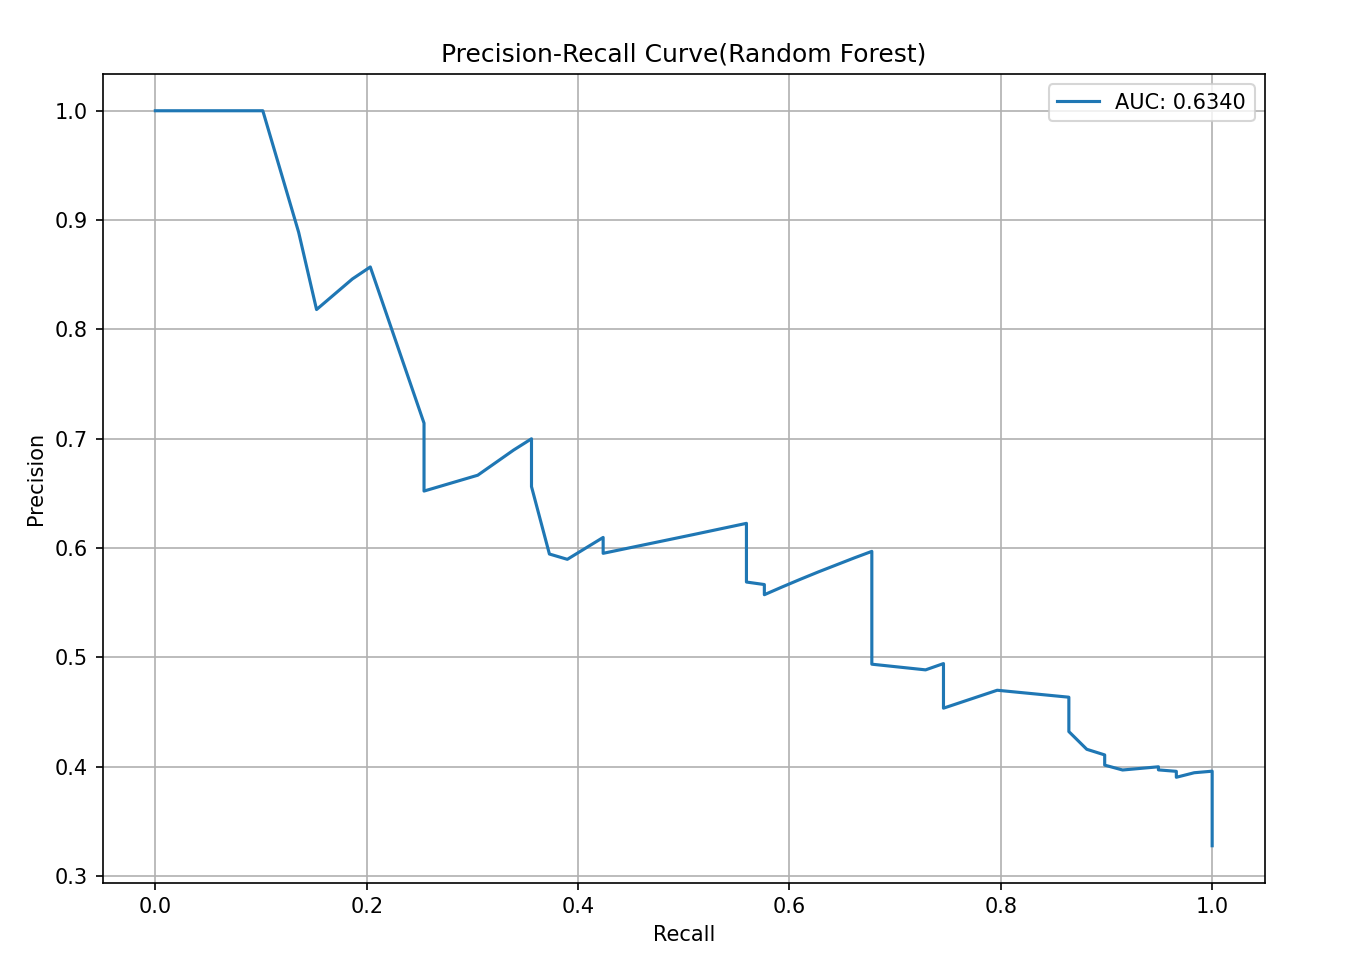
\includegraphics[width=8cm,height=6cm]{pics/7.png}
        \caption{Precision-Recall Curve}
    \end{minipage}
\end{figure}

From the confusion matrix, it can be seen that TN and TP have a large proportion compared to FP and FN, indicating a high accuracy of the model. From the Precision-Recall curve, it can be observed that the AUC is 63\%, indicating a moderate to good predictive performance of the model.

\textbf{\subsubsection{LSTM Model}}
We were not satisfied with the random forest model, so in order to further improve the prediction accuracy, we also used \textbf{the LSTM model}. LSTM is a type of long short-term memory network, which is a special type of recurrent neural network (RNN). Compared to traditional RNNs, LSTM is more suitable for handling and predicting important events with long time intervals in time series data, such as the case of heart disease patients entering the ICU with long intervals between each occurrence[5].

We used the keras library in Python to build the LSTM model. The data was also divided into a training set (80\%) and a test set (20\%), and the model was trained for 300 iterations. The results were quite good. Figure 8 shows the comparison between the predicted mortality and the actual mortality after training the LSTM model.

\begin{figure}[h]
    \centering
        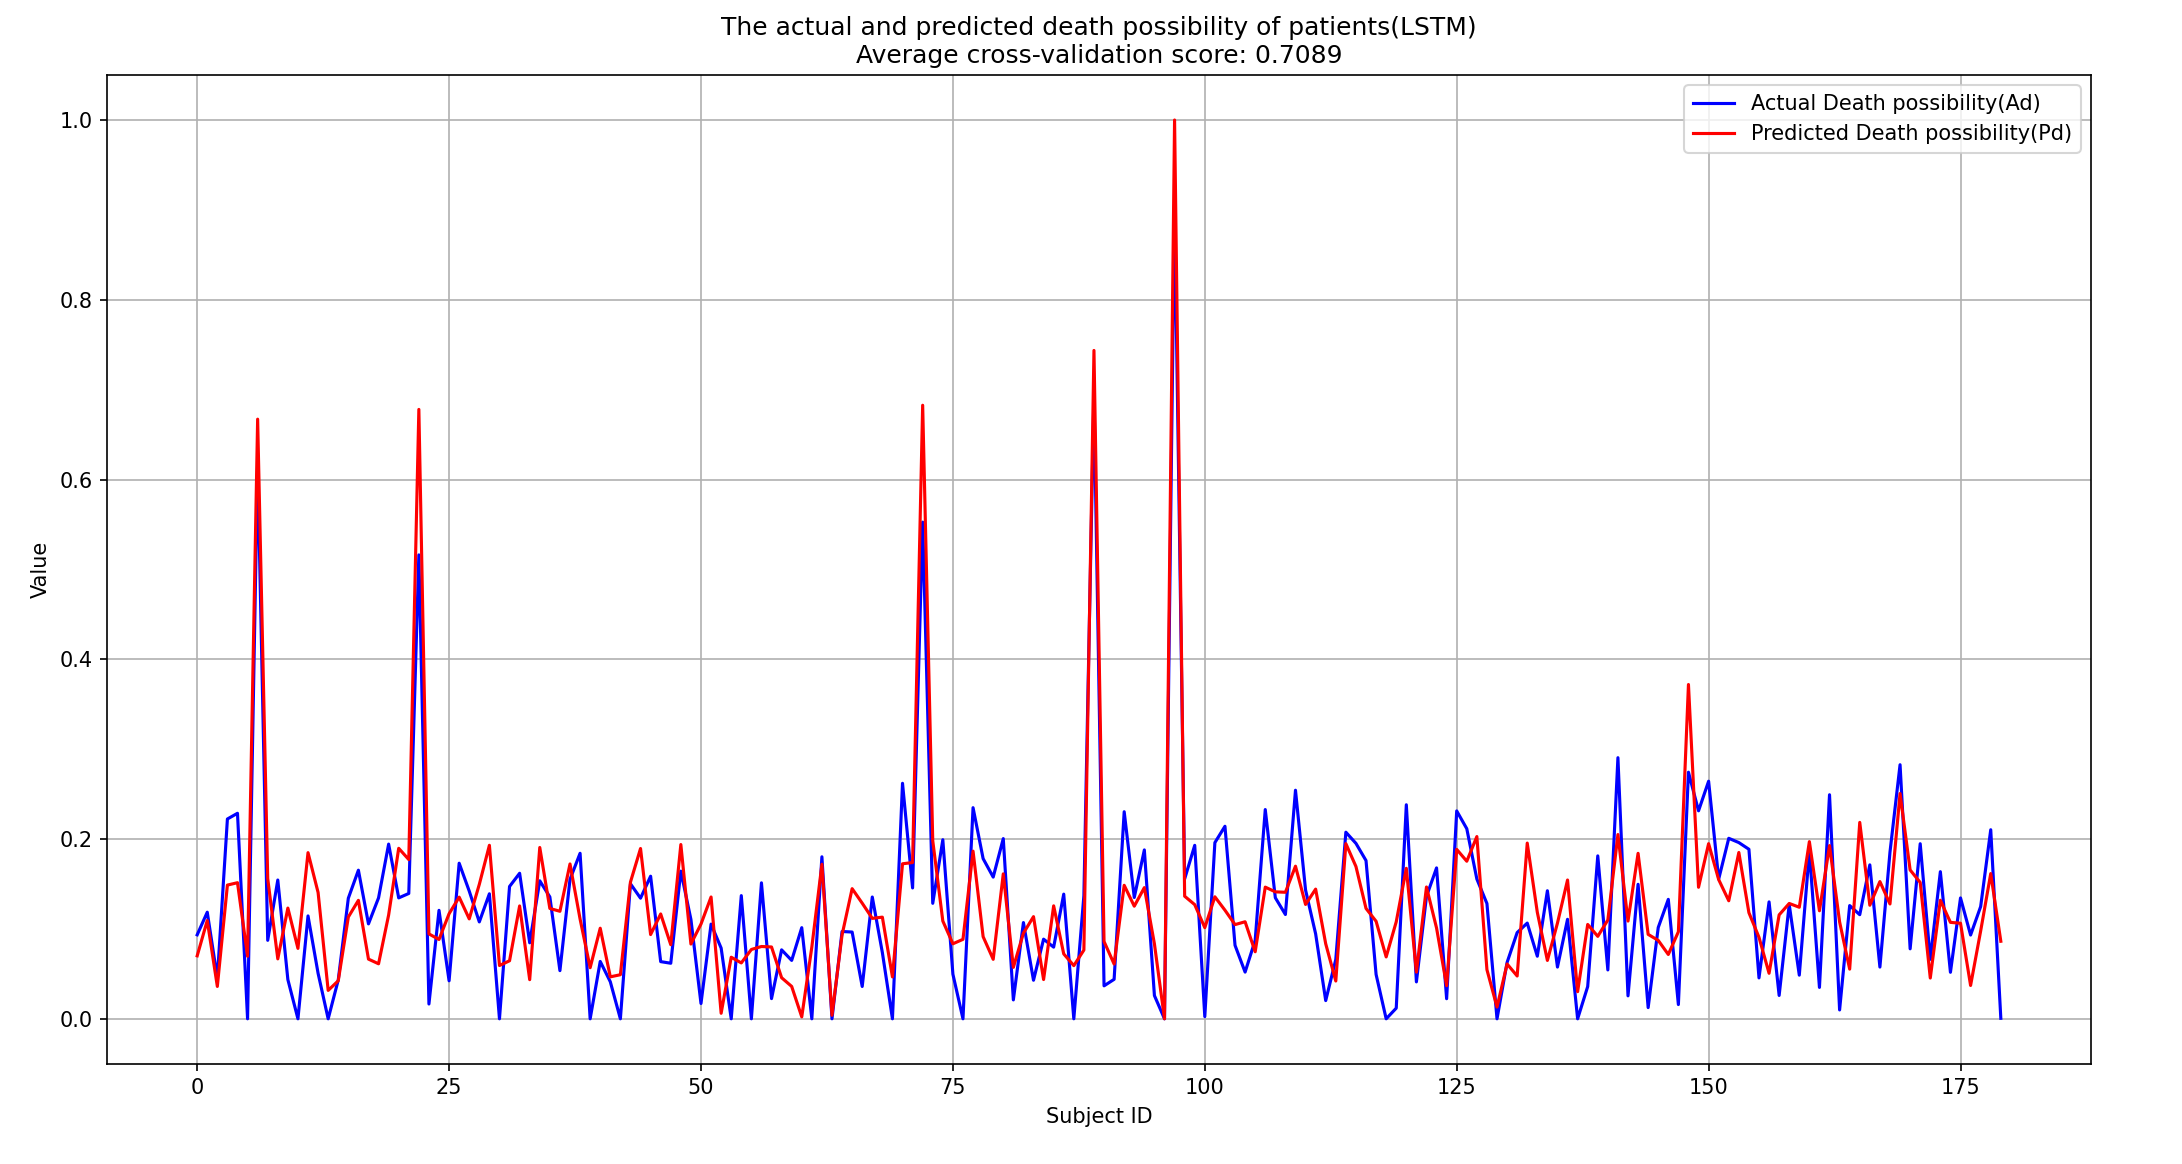
\includegraphics[width=12cm,height=6.2cm]{pics/8.png}
        \caption{The actual and predicted mortality of patients(LSTM)}
\end{figure}

The accuracy of the LSTM model reaches 71\%, showing a significant improvement compared to the random forest model. Furthermore, we also plotted the confusion matrix and Precision-Recall curve to further validate the accuracy of the model.

\begin{figure}[H]
    \begin{minipage}{0.5\textwidth}
        \centering
        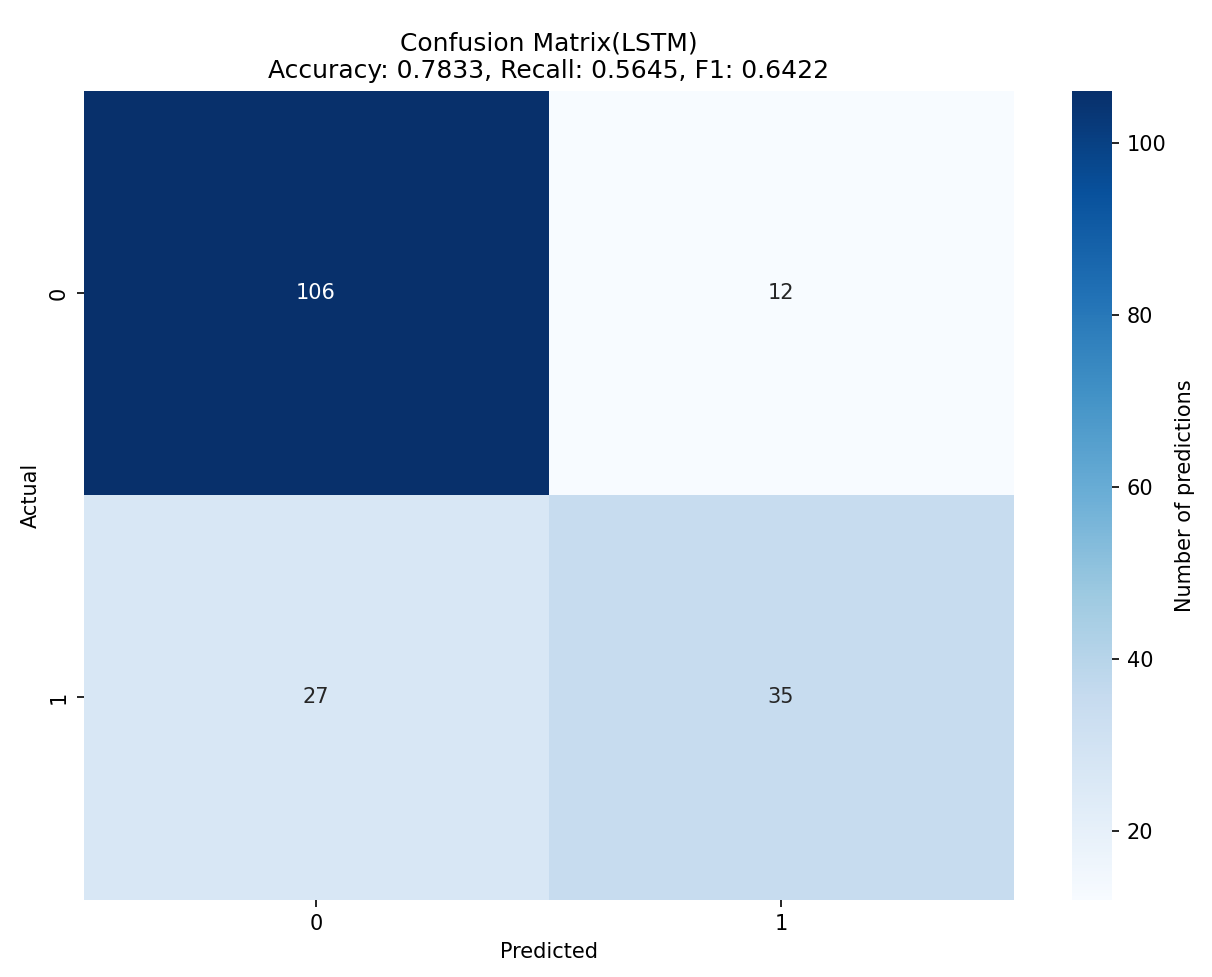
\includegraphics[width=7.5cm,height=5.6cm]{pics/9.png}
        \caption{Confusion Matrix}
    \end{minipage}
    \begin{minipage}{0.5\textwidth}
        \centering
        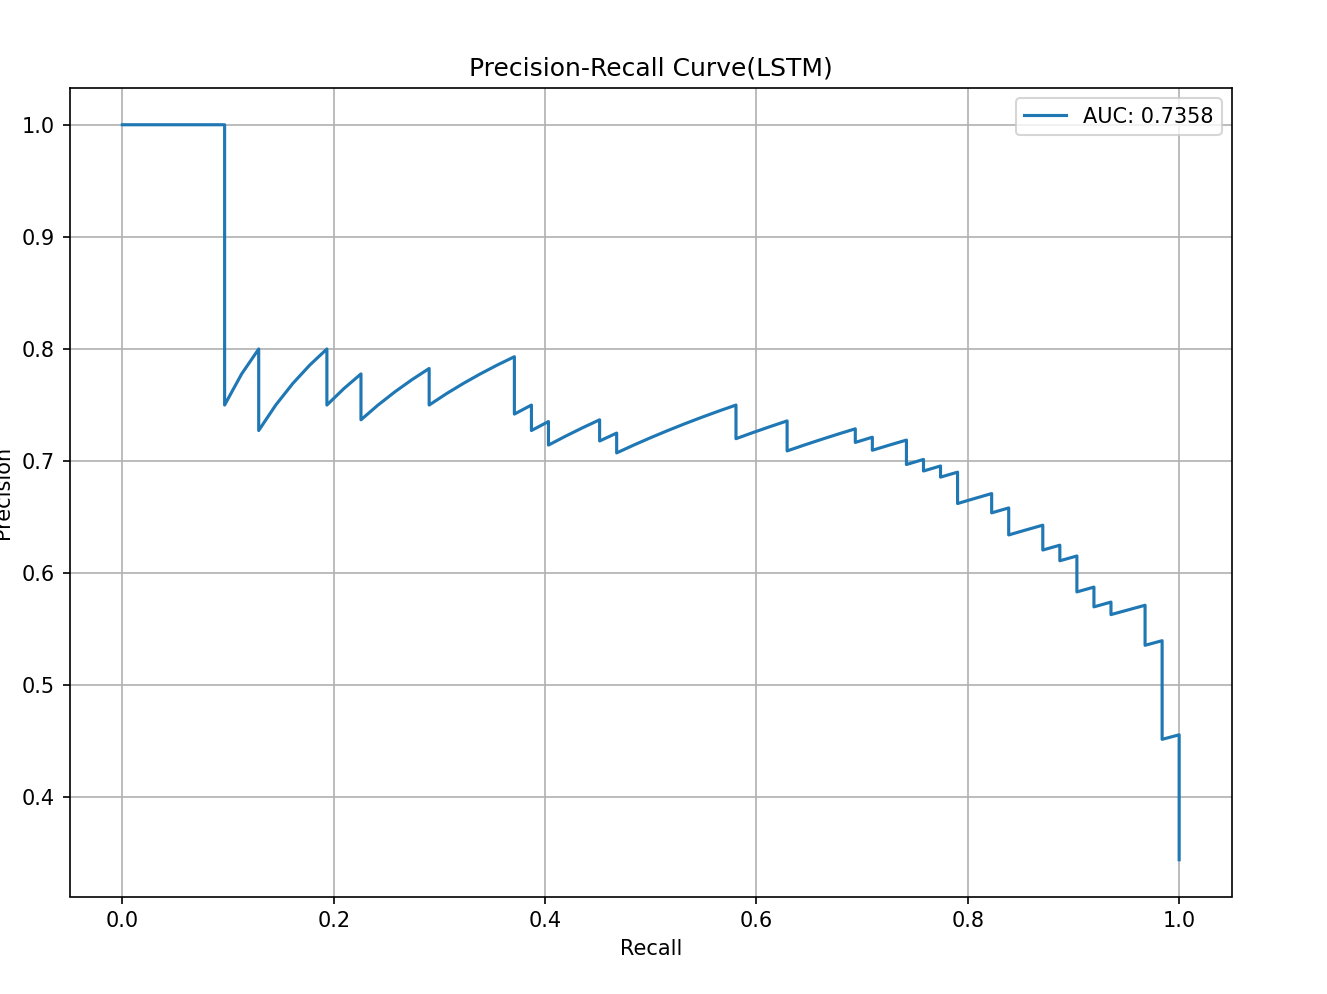
\includegraphics[width=7.5cm,height=5.6cm]{pics/10.png}
        \caption{Precision-Recall Curve}
    \end{minipage}
\end{figure}

The confusion matrix and Precision-Recall curve both indicate that the accuracy of the LSTM model approaches 75\%, which is a very gratifying achievement and also demonstrates the superiority of the LSTM model. We ultimately chose the LSTM model as \textbf{our final prediction model}.

\newpage
\textbf{\section{Strengths and Weaknesses}}
\textbf{\subsection{Strengths}}
\begin{itemize}
	\item In our model, we utilize various visualizations, including scatter plots, line charts, and heat maps, to analyze the mortality of patients suffering the heart disease. These visuals provide intuitive results for further analysis, contributing to a concise, easy-to-understand yet powerful model structure. Our model can also be applied to other diseases, such as cancer, demonstrating strong generalizability.
	\item By using the Mortality Prediction Model, our model simulates the readmission factor, predicts death, It serves as a strong alert for both heart disease patients and the healthy population.
	\item Our model boasts an impressive training speed, not only excelling in data learning but also can providing doctors with a more efficient experience, saving a significant amount of time.
\end{itemize}

\textbf{\subsection{Weaknesses}}
\begin{itemize}
    \item The model is based on the MIMIC IV dataset, which is a large, single-center database comprising information related to patients admitted to critical care units. The model may not be applicable to other datasets.
	\item We make the assumption that the data follows a hypothetical pattern. In reality, due to various influencing factors, the actual scenario might exhibit wierdly, posing the potential risk of inaccuracies in the model.
	\item Our model exhibits a heightened sensitivity to outliers, and instances where there are significantly deviant anomalies may potentially result in the instability of the model.
\end{itemize}

\newpage
\textbf{\section{Conclusion}}
We have successfully quantified the concept of "Readmission factor" to measure the mortality of patients suffering from heart disease.We have established a model to analyze and predict the mortality of patients suffering heart diseases. Which is the most important, we have achieved an accuracy of 75\% using the LSTM model to construct the prediction model.

Here are some other intriguing findings during our research:
\begin{itemize}
	\item The "Readmission factor" is not constant, but rather a dynamic value that changes with the patient's condition, so as to reflect the patient's mortality.
	\item The ICU factor has a greater impact on Mortality, while the impact of BMI is relatively small.
	\item The LSTM model is more suitable for handling and predicting important events with long time intervals in time series data, such as the case of heart disease patients entering the ICU with long intervals between each occurrence.
\end{itemize}

\textbf{\section{Suggestions to Patients}}
\begin{itemize}
    \item Patients with heart disease should pay attention to their own health and actively cooperate with the doctor's treatment.
    \item Physiologically, patients should maintain a healthy lifestyle, such as a balanced diet, regular exercise, and adequate sleep.
    \item Psychologically, patients should maintain a positive attitude, actively participate in social activities, and communicate with family and friends.
    \item Don't be too anxious about the disease, and don't be too pessimistic about the future. \textbf{Please believe that you can beat it, and we are always with you!}
\end{itemize}

% 因为不输出此部分到目录 \addcontentsline{}{}{}是添加此标题到目录 
\newpage
\textbf{\section*{References}\addcontentsline{toc}{section}{References}}
\begin{enumerate}[label={【\arabic*】}]
	\item 刘明波, 刘韫宁, 王文, 马丽媛, 周脉耕, 王黎君. 2004-2011年中国人群心血管病死亡的性别差异分析[J]. 中国慢性病预防与控制, 2014, 22 (03): 267-269.
	\item 方佳英, 陈霖祥, 唐文瑞, 林昆. 2002~2011年中国心脏病死亡的流行病学分析[J]. 汕头大学医学院学报, 2014, 27 (02): 125-127.
	\item 贺娅莎, 刘乙君, 吕定超, 李凤青, 齐昊, 王彦. 缺血性心脏病住院病人BMI与危重症风险的关系[J]. 中西医结合心脑血管病杂志, 2023, 21 (12): 2302-2304.
	\item 王羽, 刘志玄, 邱洪斌, 张艺潆. 心力衰竭重症患者院内死亡率的预测模型:基于MIMIC-Ⅲ数据库的回顾性研究[J]. 中国动脉硬化杂志, 2023, 31 (03): 245-252.
	\item 乔慧.基于数据挖掘分类技术的心脏病预测方法研究[D].导师:赵小强;王亚青.兰州理工大学,2024.
\end{enumerate}

\newpage
\textbf{\section*{Appendix: Data Processing/Statistics/Visualization Code}\addcontentsline{toc}{section}{Appendice}} 
\fontsize{13pt}{12.5pt}\selectfont

\noindent{\rule{\textwidth}{0.2mm}}
\vspace{-18pt} 
\fontsize{8pt}{7.5pt}\selectfont
{
	\lstinputlisting[language=python]{Appendix.py}
}
\vspace{-12pt}
\noindent{\rule{\textwidth}{0.3mm}}


\noindent{\rule{\textwidth}{0.3mm}}
\end{document}